\documentclass[xcolor=dvipsnames, 14pt]{beamer}
%\documentclass[xcolor=dvipsnames, bigger, aspectratio=169]{beamer}

\definecolor{Saffron}{HTML}{F4C430}
\usecolortheme[named=Saffron]{structure}

\mode<presentation> {
	\usetheme[height=2em]{Rochester}
	\setbeamercovered{transparent}
}

\setbeamertemplate{caption}{\insertcaption\par}
\setbeamertemplate{navigation symbols}{}%remove navigation symbols

\setbeamercolor{frametitle}{fg=black}
\setbeamercolor{title}{fg=black}
\setbeamercolor{navigation symbols dimmed}{fg=black!10}
\setbeamercolor{navigation symbols}{fg=black!30}
\setbeamercolor{section number projected}{fg=black}
\setbeamercolor{item projected}{fg=black}


\usepackage[utf8x]{inputenc}
\usepackage[resetfonts]{cmap}
\usepackage{lmodern}
\usepackage[czech]{babel}
\usepackage[T1]{fontenc}

\usepackage{graphicx}
\usepackage{amsmath}
\usepackage{amssymb}
\usepackage{listings}
\usepackage{microtype}
\usepackage{tikz}

\usepackage{hyperref}
\hypersetup{unicode=true}

% ----- macros -----
\newcommand{\imageW}[1]{%
  \makebox[\textwidth][c]{\includegraphics[width=1.12\textwidth]{img/#1}}}
\newcommand{\imageH}[1]{%
  \makebox[\textwidth][c]{\includegraphics[height=0.97\textheight]{img/#1}}}

% ---- info -----
\title{Adaptabilní programování}
\author{Jaroslav~Čechák \and Tomáš~Effenberger \and Jiří~Mauritz \and Barbora~Vrzáková}
\institute{Fakulta informatiky, Masarykova univerzita}
\date{\today}

\begin{document}

\begin{frame}
\titlepage
\end{frame}

\begin{frame}
\frametitle{Mise}
\begin{itemize}
\item aplikace pro efektivní učení programování
\item zábavné úlohy optimální obtížnosti
\item maximalizace \emph{flow} $\rightarrow$ efektivita + štěstí %maximalizace učení i úrovně štěstí
\end{itemize}
\end{frame}

\begin{frame}
\frametitle{Flow}
\begin{figure}[h]
  \centering
  \begin{tikzpicture}[font=\sffamily,xscale=5, yscale=5]
  \large
  %\draw [lightgray, fill=gray] (0,0) -- (0.1,0) -- (1,0.8) -- (0.8,1) -- (0,0.1) -- (0,0);
  \draw (0.1,0) -- (1,0.8);
  \draw (0,0.1) -- (0.8,1);
  \draw [thick, <->] (0,1) node [left] {obtížnost} -- (0,0) -- (1,0) node [below right] {dovednost};
  \node at (0.27,0.82) {\emph{frustrace}};
  \node at (0.6,0.6) {\emph{flow}};
  \node at (0.7,0.2) {\emph{nuda}};
  \end{tikzpicture}
  %\caption{Relationship between challenge and skill.}
\end{figure}
\end{frame}

\begin{frame}
\frametitle{Letní prototyp}
\imageW{practice.png}
\end{frame}

\begin{frame}
\frametitle{Úlohy}
\imageH{task-example.png}
% NOTE: ulohy muzou obsahovat klice, jamy, barvy
\end{frame}

\begin{frame}
\frametitle{Koncepty a instrukce}
\imageW{first-problem.png}
\end{frame}

\begin{frame}
\frametitle{Konečné tréninky}
\imageW{advanced-problem.png}
\end{frame}

\begin{frame}
\frametitle{Motivace a interpretace: kredity}
\imageW{task-completion-modal.png}
\end{frame}

\begin{frame}
\frametitle{Motivace a interpretace: bloky}
\imageW{statistics-blocks.png}
\end{frame}

\begin{frame}
\frametitle{Statistiky}
\imageW{statistics-overview.png}
\end{frame}

\begin{frame}
\frametitle{Statistiky}
\imageW{statistics-solved-tasks.png}
\end{frame}

\begin{frame}
\frametitle{Admin statistiky}
\imageW{admin-stats.png}
\end{frame}

\begin{frame}
\frametitle{Přihlašování přes Google/Facebook}
\imageW{social-auth.png}
\end{frame}

\begin{frame}
\frametitle{Anglická lokalizace}
\imageW{localization.png}
\end{frame}

\begin{frame}
\frametitle{HTTPS}
\centering

\includegraphics[width=0.5\textwidth]{img/https.png}
\end{frame}

\begin{frame}
\frametitle{Sbírání a export dat}
\imageW{data-export.png}
\end{frame}

\begin{frame}
\frametitle{Plán -- podzim 2016}
\begin{itemize}
\item refaktoring jádra
\item refaktoring backendu
\item refaktoring frontendu
\item intuitivní uživatelské rozhraní
\item téma, nové úlohy, grafika
\item iniciální analýzy
\end{itemize}
\end{frame}

\begin{frame}
\frametitle{Téma -- požadavky}
\begin{itemize}
\item zábavné pro děti
  % pro kluky i holky, a rozumne i pro starsi (ale do budoucna zajimavy namet k adaptabilite)
\item potenciál pro velkou spoustu zajímavých úloh
  % ulohy musi byt vyzvou a byt "pekne"
  % vcetne (zejmena) tech opravdu jednoduchych (hlavni problem aktualniho tematu)
  % <- malé množství ortogonálních prvků
\item stručnost programů
  % pokud jde myslenku zachytit 4 bloky, mely by stacit 4 bloky
  % minimalizace boilerplatu
\item neomezovat adaptabilitu
  % napr. pribehem
  % obecne ne na ukor vyzkumnych otazek
\item možnost rozvíjet další témata
  % nechat si otevrene dvere pro slozitejsi koncepty
  % nebo kdyz nam dojdou napady na zajimave ulohy nebo budeme chtit vyzkouset ruzna temata kvuli vyzkumu)
\end{itemize}
\end{frame}

\begin{frame}
\frametitle{Téma: Raketka}
\begin{itemize}
\item akce: pohyb a střílení
\item limit: bloky (kroky) a munice
\item políčka: podklad a objekt
\item podmínky: kontrola podkladu a pozice
\item příkazy, cykly, funkce, větvení, logické výrazy
\end{itemize}
\centering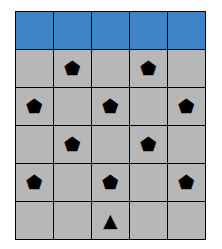
\includegraphics[width=0.3\textwidth]{img/raketka.png}
\end{frame}

\begin{frame}
\frametitle{Uživatelské rozhraní: draft}
\imageW{new-user-interface-1.png}
\end{frame}

\begin{frame}
\frametitle{Uživatelské rozhraní: draft}
\imageW{new-user-interface-2.png}
\end{frame}


\begin{frame}
\frametitle{Architektura -- požadavky}
\begin{itemize}
\item sdílení kódu mezi webem a analýzami
  % např. modely, ale i vizualizace
\item inteligentní analýzy, rozumné jádro a hloupý web
  % web ani nemusi vedet, co ktera akce znamena za zmeny stavu
\item systematické sbírání dat o všech akcích
  % provedeni akce by automaticky melo znamenat jeji ulozeni, misto aktualniho proved a zaloguj
\item snadnost ladění -- cestování v čase, vizualizace
  % zejm. chyb na produkci, ale i behem vyvoje (a tyka se i vizualizacnich komponent)
  % taky nemuset vyklikavat posloupnosti akci
\item kód je radost číst, psát a testovat % proste tvori nadherny pribeh, ve kterem je snadne se zorientovat, cist ho, rozsirovat ho, ladit chyby, testovat
\end{itemize}
\end{frame}

\begin{frame}
\frametitle{Architektura -- návrh}
\begin{itemize}
\item čisté jádro
  \begin{itemize}
  \item model světa: stav, akce, redukce
      % uvest priklady
      % stav - entity a kontext
      % akce a redukce jsou ortogonalni koncepty
  \item extraktoři (techniky, statistiky, \ldots)
  \item statická data
  \item komponenty pro vizualizaci
    % ReactJS + redux architecture
    % ES6 - v nekterych ohledech dokonce lepsi nez Python!
  \end{itemize}
\item web  % backend i frontend, zatim pohodlna tesna vazba
  \begin{itemize}
  \item obaluje jádro, řeší IO
    % frontend, persistence v DB, autentizace, posilani mailu, ...
  \item nemusí znát logiku akcí
    % ale musi znat jejich semantiku - kdy ma kterou spustit
  \item poskytuje a ukládá stav světa a akce
  \end{itemize}
\item analýzy
\end{itemize}
\end{frame}

\begin{frame}
\frametitle{Odkazy}
\begin{itemize}
\item prototyp:
  \begin{itemize}
  \item \footnotesize{\url{https://robomise.cz}}
  \end{itemize}
\item repozitáře:
  \begin{itemize}
  \item \footnotesize{\url{https://github.com/adaptive-learning/flocs}}
  \item \footnotesize{\url{https://github.com/adaptive-learning/flocs-core}}
  \item \footnotesize{\url{https://github.com/adaptive-learning/flocs-web}}
  \end{itemize}
\end{itemize}
\end{frame}

\end{document}
